\documentclass{beamer}

\usepackage[ngerman]{babel}
\usepackage[utf8x]{inputenc}
\usepackage{amsmath,amsfonts,amssymb}
\usepackage{tikz}
\usepackage{graphicx}
\usepackage{eurosym}

\usetikzlibrary{shapes,arrows,positioning,hobby,decorations.markings,fit,backgrounds,calc}

%\usetheme{Singapore}
\setbeamercovered{transparent}

\setbeamertemplate{section in toc}[sections numbered]
\setbeamertemplate{subsection in toc}[subsections numbered]
\setbeamertemplate{subsubsection in toc}[subsubsections numbered]

\newcommand{\btVFill}{\vskip0pt plus 1filll}

\newcommand\subsectnum{%
  \number\numexpr \insertpagenumber-\insertsubsectionstartpage+1\relax.~%
}

\begin{document}
\title{IOT - Remote}   
\author{Eike Florian Petersen / Michael H}
\date{\today}

\frame{\titlepage

\begin{minipage}{-0mm}
\hspace*{-1.3cm}
  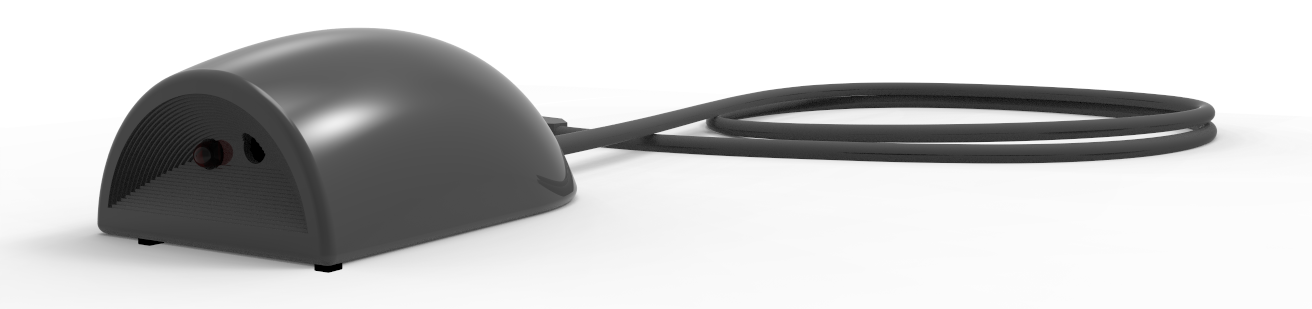
\includegraphics[width=13.5cm]{1_title}
\end{minipage}
}

\frame{\frametitle{Inhaltsverzeichnis}\tableofcontents} 


\section {Einleitung}
\subsection*{Motivation}
\frame {\frametitle{\thesection.\thesubsection~\insertsection~- \insertsubsection}
\begin{itemize}
	\item Entwicklung frei konfigurierbare IoT-Infrarot Schnittstelle/Fernbedingung
	\item Günstige Lösung im Vergleich zu einer teuren programmierbaren Fernbedingung
	\begin{itemize}
		\item $\rightarrow$ Logitech MyHarmony (aktuell \EUR{129,00})
	\end{itemize}
	\item Steuerung über verschiedener Endgeräte (Tablet, Handy, PC,..) per Browser
\end{itemize}

%Es soll eine frei konfigurierbare IoT-Infrarot Schnittstelle entstehen, welche außer dem Sender und seiner Stromversorgung keine weitere zusätzliche Hardware benötigt. Das erstrebte Ziel hebt sich von älteren Produkten der Firma Logitech aufgrund seiner nicht benötigten zweiten Hardwarekomponente (Fernbedienung) ab. Gleiches strebt auch Logitech mit dem MyHarmony Hub (aktuell \EUR{129,00}) an.\\
}

\subsection*{Aufgaben}
\frame {\frametitle{\thesection.\thesubsection~\insertsection~- \insertsubsection}
\begin{itemize}
	\item WiFi Einstellungen hinterlegen
	\item Fallback in AP Modus
	\item Webserver
	\item Steuerung des ESP8266 über Website (Feedback)
	\item Erfassen, Speichern und Ausgabe von Infrarot-Signalen (38kHz)
\end{itemize}
}
% Häufige Probleme mit dem Hub und der IOs / Android Anwendung, so wie später auslaufender Support von bestimmten Versionen von iOS und Android wird durch das Nutzen eines Webservers vorgebeugt

\section {Bauteilliste}
\frame {\frametitle{\thesection.~\insertsection}
\begin{itemize}
	\item Mikrocontroller: ESP8266
	\item linearer Spannungsregler: LM1117-3V3 \\ (4.75V - 10V, max. 800 mA $\rightarrow$ 3.3V)
	\item Zwei Kondensatoren: 10 $\mu$F, 100nF
	\item IR-Diode: 1,5V / 80mA
	\item Vorwiderstand für IR-Diode: 22 Ohm
	\item IR-Fotodiode: TSOP4838 für die Trägerfrequenz 38kHz \\ (TSOP48.. in 30, 33, 36, 36.7, 38, 40, 50kHz)
	\item USB-to-UART-Programmierer: PL2303 \\ (Vss-Out = 5V)
\end{itemize}
}

\section {Schaltplan}
\frame {\frametitle{\thesection.~\insertsection}
\begin{minipage}{-0mm}
  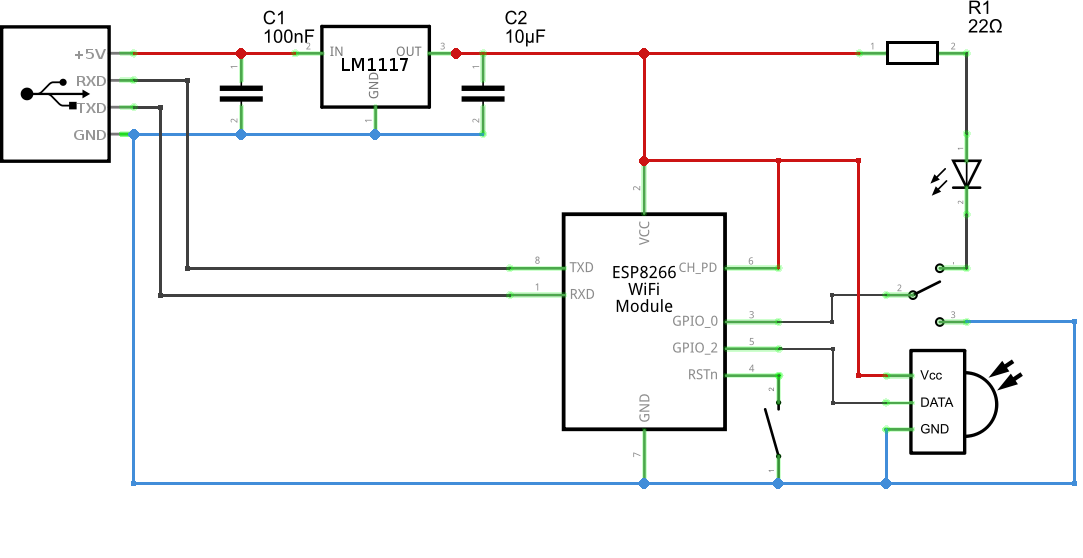
\includegraphics[width=11cm]{3_circuit_layout}
\end{minipage}
}

\section {Programm}
\subsection*{EEPROM}
\frame {\frametitle{\thesection.\thesubsection~\insertsection~- \insertsubsection}
Lesen :\\
~ EEPROM.read(bytenr);\\~\\
Schreiben:\\
~ EEPROM.write(bytenr, 0);\\
~ EEPROM.write(bytenr, value);\\
~ \\
\begin{tikzpicture}
%Erster Block
\draw (0,0) -- (1,0) (1,1) --  (0,1) -- (0,0);
\draw (2,0) -- (3,0)  -- (3,1) --  (2,1);
\draw[loosely dotted] (2,1) -- (1,1);
\draw[loosely dotted] (2,0) -- (1,0);
\node[text width=4cm] at (2.4,1.2) {0};
\node[text width=4cm] at (4.3,1.2) {96};
\node[text width=4cm] at (2.5,0.45) {WiFi-Settings};
%Zweiter Block
\draw (4,0) -- (5,0) -- (5,1) --  (4,1) -- (4,0);
\draw (5,0) -- (6,0)  (6,1) --  (5,1) -- (5,0);
\draw (7,0) -- (8,0)  -- (8,1) --  (7,1);
\draw[loosely dotted] (6,1) -- (7,1);
\draw[loosely dotted] (6,0) -- (7,0);
\node[text width=4cm] at (6.2,1.2) {150};
\node[text width=4cm] at (7.2,1.2) {151};
\node[text width=4cm] at (9.2,1.2) {4095};

\node[text width=4cm] at (6.05,0.45) {\footnotesize Anzahl};
\node[text width=4cm] at (7.7,0.45) {IR-Codes};
% Detailansicht von IR-Codes

\draw (1,-2) -- (2,-2) -- (2,-1) --  (1,-1) -- (1,-2);
\draw (2,-2) -- (3,-2)  (3,-1) --  (2,-1) -- (2,-2);
\draw (4,-2) -- (5,-2)  -- (5,-1) --  (4,-1);
\draw[loosely dotted] (3,-1) -- (4,-1);
\draw[loosely dotted] (3,-2) -- (4,-2);
\node[text width=4cm] at (3.05,-1.55) {\footnotesize Anzahl};
\node[text width=4cm] at (4.2,-1.55) {\footnotesize ~ ~ ~ ~Name \\ (1 Byte / Zeichen)};
\draw (5,-2) -- (6,-2) -- (6,-1) --  (5,-1) -- (5,-2);
\draw (6,-2) -- (7,-2)  (7,-1) --  (6,-1) -- (6,-2);
\draw (8,-2) -- (9,-2)  -- (9,-1) --  (8,-1);
\draw[loosely dotted] (7,-1) -- (8,-1);
\draw[loosely dotted] (7,-2) -- (8,-2);
\node[text width=4cm] at (7.05,-1.55) {\footnotesize Anzahl};
\node[text width=4cm] at (8.6,-1.55) {\footnotesize ~ ~ Zeiten \\ (2 Byte / Int)};
\draw[loosely dotted] (9,-1) -- (10,-1);
\draw[loosely dotted] (9,-2) -- (10,-2);

%Verbindungen
\draw (5,0) -- (1,-1);
\draw (8,0) -- (10,-1);

\end{tikzpicture}
%	\item 0 - 96 = WLAN-Daten
%	\item 97 - 149 = Vorgehalten für weitere Einstellungen
%	\item 150 = Stationsanzahl bzw. Anzahl der gespeicherten Infrarotcodes
%	\item 151 - 4095 = Stationen bzw. Infrarotcodes
}

\subsection*{Infrarot}
\frame {\frametitle{\thesection.\thesubsection~\insertsection~- \insertsubsection}
Lesen:\\
\begin{itemize}
	\item Abgreifen mit 38 kHz (26.3 $\mu$s / Takt) mit 10.000 Abgriffen $\rightarrow$ 263 ms.
	\item Gespeichert werden nur die Flankenwechsel mit der jeweiligen Abgriffsnummer.\\
	Vorteil: Int (2 Byte), geringe Anzahl
\end{itemize}
%TODO : Beispiel Einfügen


Wiedergeben:\\
\begin{itemize}
	\item Emulieren von Signalen, welche auf eine Trägerfrequenz von 38kHz moduliert sind.
	\item 1Takt $\rightarrow$ 13.15 $\mu$s High, 13.15 $\mu$s Low
\end{itemize}
%TODO : Beispiel Einfügen

}

\subsection*{Webserver}
\frame {\frametitle{\thesection.\thesubsection~\insertsection~- \insertsubsection}
\begin{minipage}{0.49\textwidth} 
\begin{itemize}
\item Setup( )
\begin{itemize}
	\item Lese Daten aus Speicher
	\item Starte Modus
\end{itemize}
\item Loop( )
\begin{itemize}
	\item Verarbeite Anfragen von IP-Adresse oder \url{iot_remote.local} (mDNS)
	\item Rufe entsprechende Funktionen auf (z.B. Infrarotcodes aufnehmen)
	\item Liefere Website aus	
\end{itemize}

\end{itemize}
\end{minipage}
\hfill
\begin{minipage}{0.49\textwidth}

% Define block styles
\tikzstyle{decision} = [diamond, draw, 
    text width=4.5em, text badly centered, node distance=3cm, inner sep=0pt]
\tikzstyle{block} = [rectangle, draw, 
    text width=5em, text centered, rounded corners, minimum height=4em]
\tikzstyle{line} = [draw, -latex']
\tikzstyle{cloud} = [draw, ellipse, node distance=3cm,
    minimum height=2em]

\begin{tikzpicture}[node distance = 2cm, auto, scale=0.5, every node/.style={scale=0.8}]
    % Place nodes
    \node [block] (connectWLAN) {Verbinde mit WLAN};
    \node [decision, below of=connectWLAN] (decide) {Erfolgreich ?};
   	\node [block, left of=decide, node distance=4cm] (startAP) {Starte als AP};
    \node [block, below of=decide, node distance=3cm] (mDNS) {Starte mDNS};
 	\node [block, below of=mDNS] (launch) {Starte Server};

    % Draw edges

    \path [line] (connectWLAN) -- (decide);
	\path [line] (decide) -- node [near start] {Nein} (startAP);
    \path [line] (startAP) |- (launch);
    \path [line] (decide) -- node {Ja}(mDNS);
    \path [line] (mDNS) -- (launch);
\end{tikzpicture}
\end{minipage}
}

\section{Fazit}
\subsection*{Probleme bei der Umsetzung}
\frame {\frametitle{\thesection.\thesubsection~\insertsection~- \insertsubsection}
%TODO :Es befüllen
	\begin{itemize}
		\item dynamisch zugewiesene IP-Adresse im WLAN 
		\begin{itemize}
			\item $\rightarrow$ einfacher Zugriff per mDNS
		\end{itemize}
		\item schwieriges Debuggen, da alle Pins belegt %TODO Diese Aussage okay? -> Weil GPIO nicht auf low liegt... 
		\begin{itemize}
			\item $\rightarrow$ nur möglich, wenn GPIO\_0 auf Low liegt
		\end{itemize}
	\end{itemize}
}

\subsection*{Aufgabenverteilung}
\frame {\frametitle{\thesection.\thesubsection~\insertsection~- \insertsubsection}
Michael\\
\begin{itemize}
	\item WLAN Einstellungen, Fallback in AP-Modus, mDNS
	\item EEPROM Schreiben, Lesen
	\item Dokumentation
\end{itemize}  
Eike\\
\begin{itemize}
	\item Elektronische Schaltung
	\item IR Empfang, Speichern, Senden
	\item HTML-Layout
\end{itemize} 
}

\subsection*{Ergebnis}
\frame {\frametitle{\thesection.\thesubsection~\insertsection~- \insertsubsection}
%TODO :Es befüllen
\begin{itemize}
	\item Programmierbare IoT-Fernbedingung realisiert
	\item $\rightarrow$ kostengünstig %als Logitech Harmony!! 
	\item Zugriff über verschiedenste Endgeräte möglich %Notebook, Handy, Tablet, PC....
	\item Code und Dokumentation abrufbar unter: \url{https://github.com/Ava-chan/IOT_IR_Remote}
\end{itemize}
}

\section {Live Demo}
\frame {\frametitle{\thesection.~\insertsection}
\begin{minipage}{-0mm}
\hspace*{-1.3cm}
\vspace*{4.0cm}
  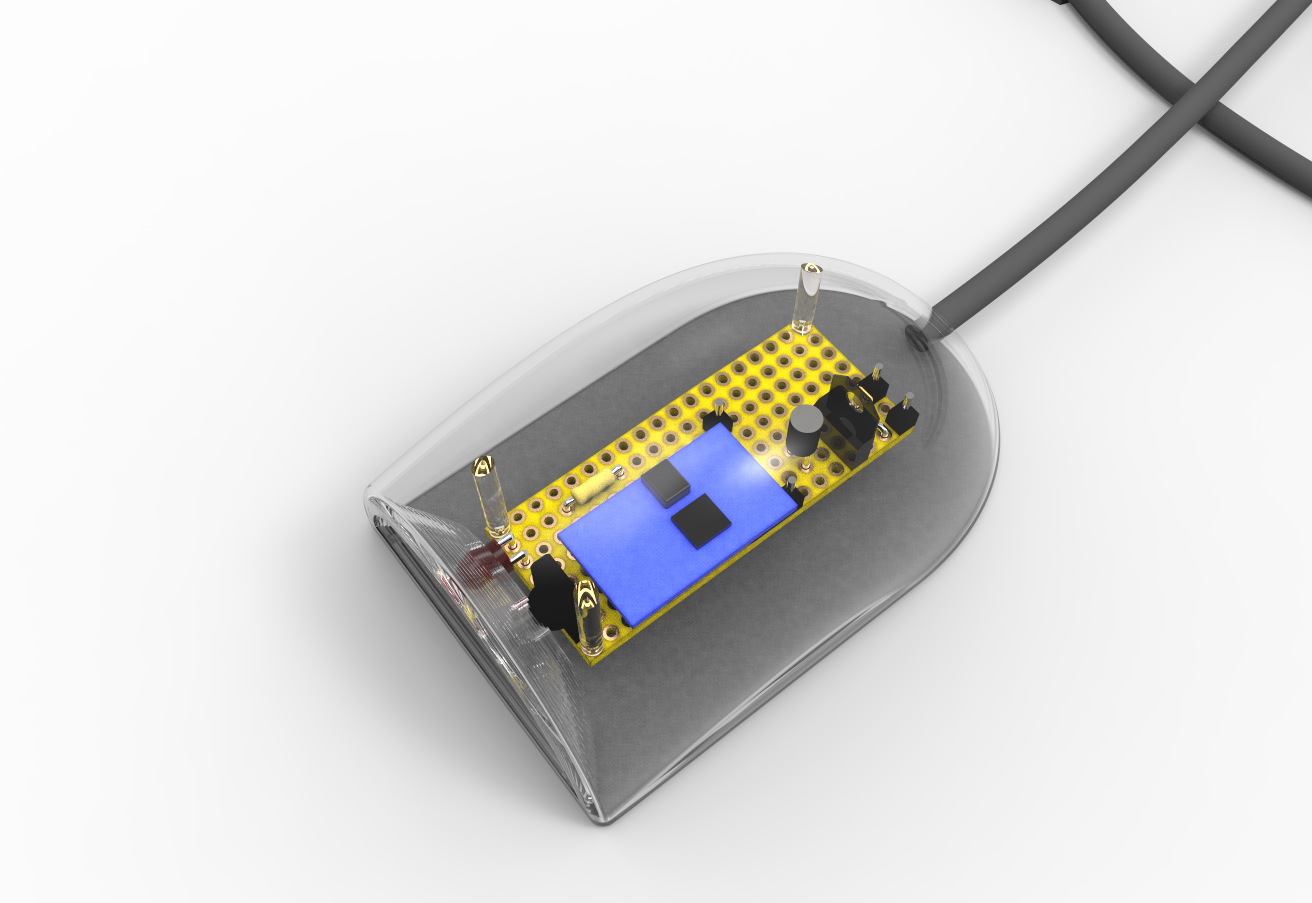
\includegraphics[width=13cm]{7_Live_Demo}
\end{minipage}
}

\end{document}


